%!TEX root = userguide.tex
\section{Downloading and Compiling PEBBL}
\label{sec:downloadcompile}

\subsection{System requirements}
\begin{itemize}
\item A Unix-like operating systems (including Linux, Mac OS X, or some
version of the Linux subsystem for Microsoft Windows).  This guide assumes
basic familiarity with the command-line interface to such environments.
\vspace{-1.8ex}
%% Make below optional if tarballs can be used
\item The \texttt{git} version management system (required for initial download only)
\vspace{-1.8ex}
\item The \texttt{cmake} configuration and build system (including GNU \texttt{make})
\vspace{-1.8ex}
\item A C++ compiler, such as g++
\vspace{-1.8ex}
\item For parallel execution, some form of MPI, such as OpenMPI or MPICH.
\end{itemize}
These packages should be readily installable in most Unix-like
systems.  

The PEBBL distribution also includes some Python scripts, for which a Python
interpreter is needed.  These scripts perform auxiliary functions and are not
required to run PEBBL.


\subsection{Downloading PEBBL}
To download the latest version of PEBBL, issue the following \texttt{git} command:
{\small
\begin{codeblock}
git clone https://github.com/PEBBL/pebbl.git
\end{codeblock}
}
\noindent This command will create a directory called
\texttt{pebbl}.  


\subsection{Configuration}
\label{sec:compile}
\label{sec:compiling}
PEBBL now uses \texttt{cmake} and an ``out-of-source'' build scheme.  To
configure PEBBL for your system, create another directory at the same level as
the \texttt{pebbl} directory created by \texttt{git}; this directory will hold
your compiled version of PEBBL.  From here on, this document will assume that
this directory is called \texttt{buildpebbl}, but the name can be anything you
wish.

Before compiling, you must configure PEBBL.  To do so, first descend into the
\texttt{buildpebbl} directory.  If you are in an environment with usable X
graphics, then give the command
\begin{codeblock}
cmake-gui ../pebbl
\end{codeblock}
If your system does not have usable X graphics (for example, if running over a
slow remote connection) then instead give the command
\begin{codeblock}
ccmake ../pebbl
\end{codeblock}

\subsubsection{Configuring with \texttt{cmake-gui}}
After you start \texttt{cmake-gui}, a window like the one shown in
Figure~\ref{fig:cmake1} should appear.  Start the configuration process by
pressing the "Configure" button on the lower left, after which a window like
that in Figure~\ref{fig:cmake-choosegen} should pop up.

\begin{figure}[tpb]
\begin{center}
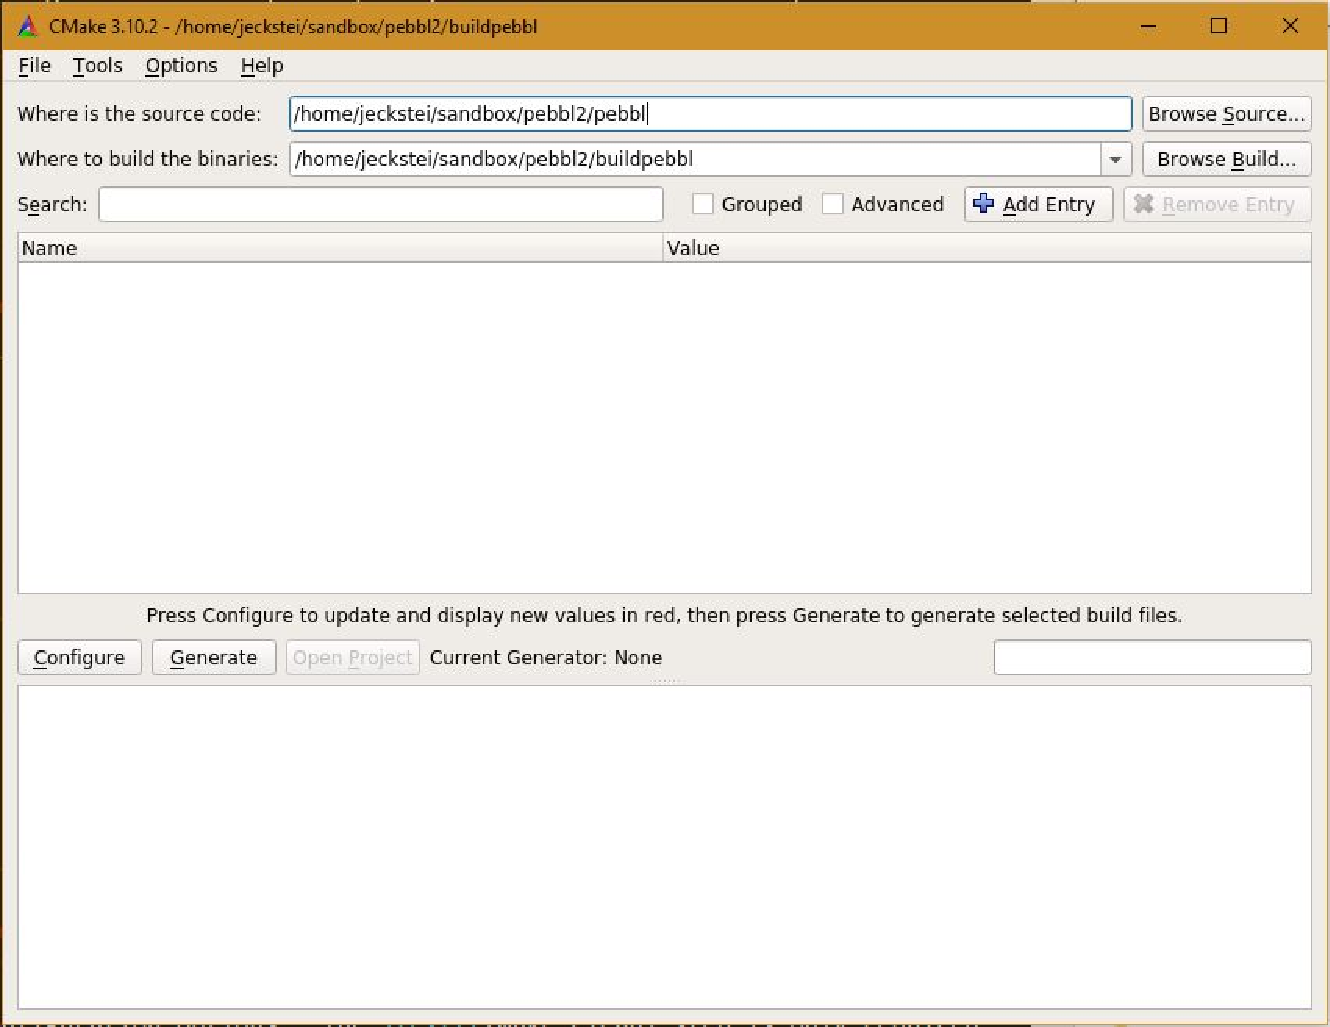
\includegraphics[height=0.45\textheight]{cmake1}
\vspace{-0.3in}
\end{center}
\caption{Initial display from \texttt{cmake-gui}.\label{fig:cmake1}}
\end{figure}

\begin{figure}[tpb]
\begin{center}
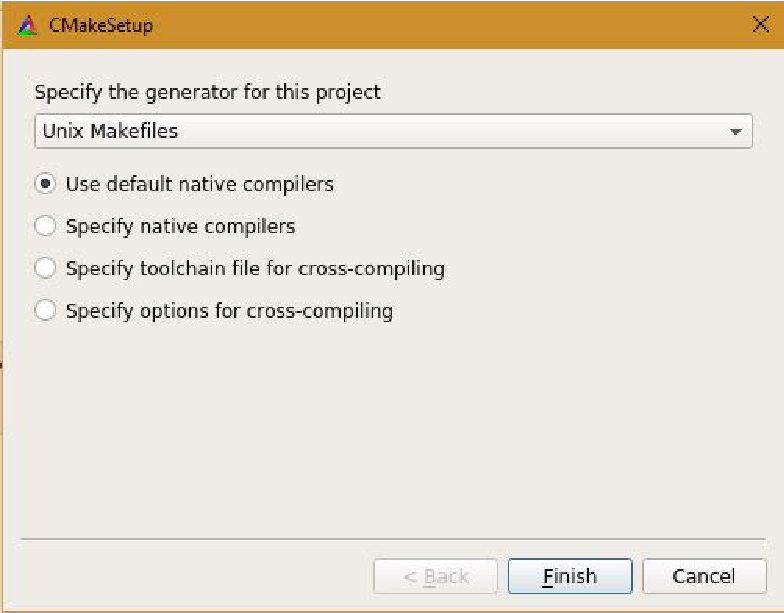
\includegraphics[width=0.45\textwidth]{cmake-choosegen}
\vspace{-0.3in}
\end{center}
\caption{Generator choice pop-up from \texttt{cmake-gui}.\label{fig:cmake-choosegen}}
\end{figure}

For ordinary applications, it is sufficient to press the ``Finish'' button in
this pop-up window, which selects the default native compilers.  If you wish
to specify a non-default C++ compiler or use a cross-configuration
environment, you may select one of the other options.  This guide covers only
the default native case.

The next display from \texttt{cmake-gui} should resemble
Figure~\ref{fig:cmake2}.  You should now select the build options you desire
by modifying the entries in the "Value" column of this display.

\begin{figure}[tpb]
\begin{center}
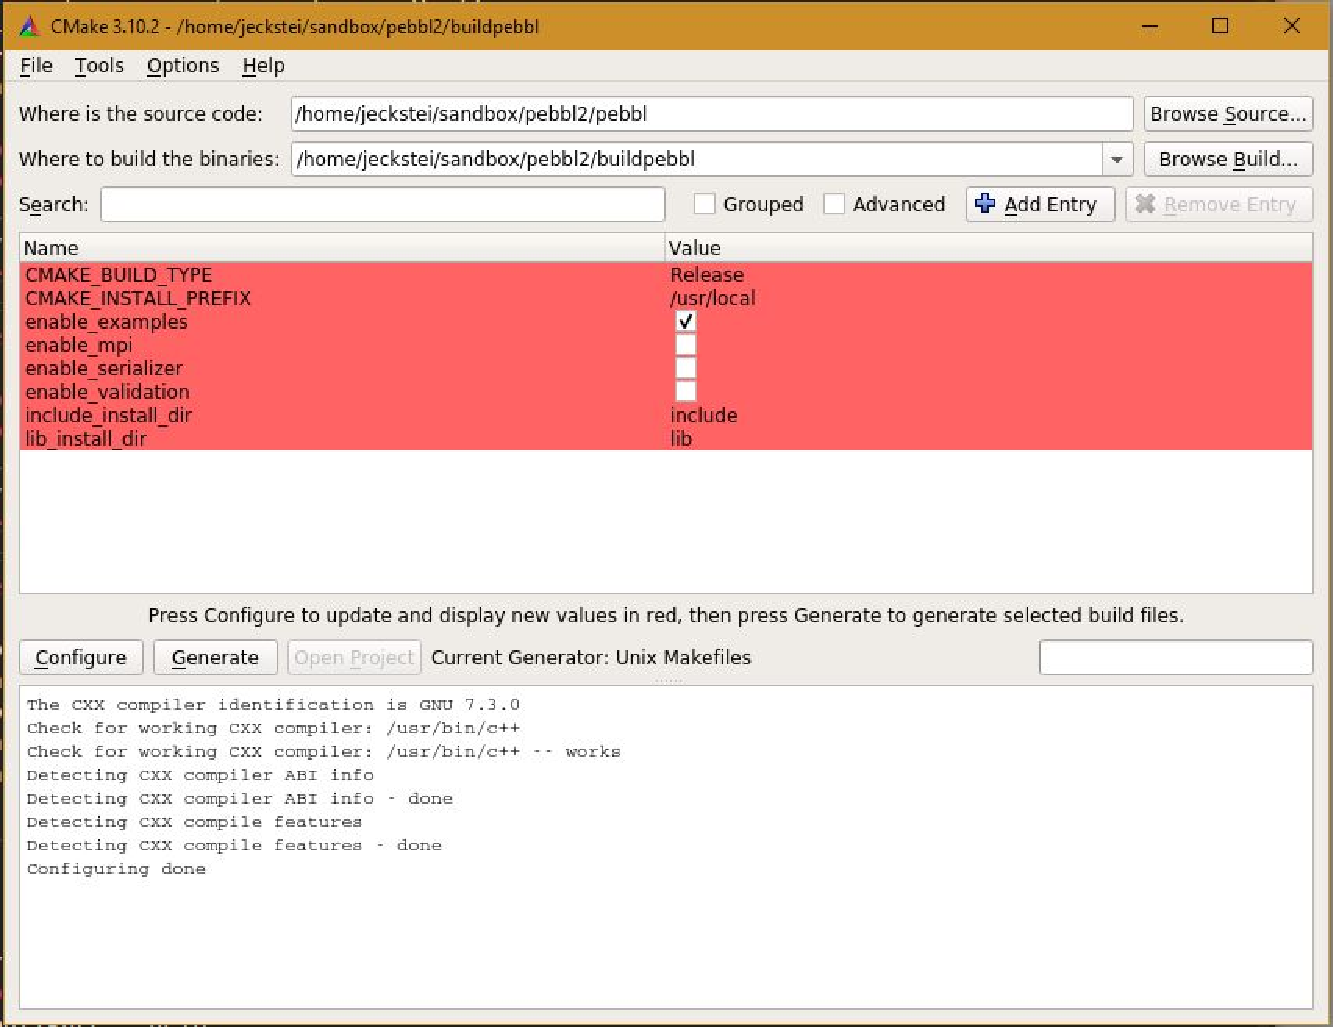
\includegraphics[height=0.45\textheight]{cmake2}
\vspace{-0.3in}
\end{center}{}
\caption{Appearance of \texttt{cmake-gui} after initial configuration step.
  \label{fig:cmake2}}
\end{figure}

\begin{description}
\item[\texttt{CMAKE\_BUILD\_TYPE}:] The default value ``Release'' builds a
version of PEBBL with compiler optimization and without symbol table
information.  You may change this to ``Debug'' to build a version with symbol
table information (the \texttt{-g} option in many compilers).  A ``Debug''
version will be somewhat slower but allow symbolic debuggers such as
\texttt{gdb} to view PEBBL's internal code.  You may still compile your own
application with debugging information, but compile PEBBL itself in
``Release'' mode.
\item[\texttt{CMAKE\_INSTALL\_PREFIX}:] Specifies where the command
\texttt{make install} will attempt to install the PEBBL headers and library.
\item[\texttt{enable\_examples}:]  Leave checked to build the sample
applications that come with PEBBL, or uncheck to build only the PEBBL library.
The sample applications can be useful in verifying that PEBBL was built
successfully. 
\item[\texttt{enable\_mpi}:]  Check this box to build both the parallel and
serial layers, which requires a version of MPI.  If you leave this box
unchecked, only the serial layer will be built, with the modules in the
parallel layer treated as ``stubs''.  See Section~\ref{sec:arch},
page~\pageref{sec:arch} for an explanation of the distinction between the
serial and parallel layers.
\item[\texttt{enable\_serializer}:]  This option should ordinarily be left
unchecked.  It enables some utility functions that may slightly improve
performance but are not compatible with the recent C++ compilers.
\item[\texttt{enable\_validation}:]  Enables some internal error-checking
functions that may have a small negative impact on run-time performance.
\item[\texttt{include\_install\_dir:}] This option controls the location of
header files within the specified \texttt{CMAKE\_INSTALL\_PREFIX} directory.
It should ordinarily be left unchanged.
\item[\texttt{lib\_install\_dir:}] This option controls the location of the
PEBBL object library within the specified \texttt{CMAKE\_INSTALL\_PREFIX} directory.
It should ordinarily be left unchanged.
\end{description}
A host of additional options are available by checking the ``Advanced'' box
above the option table.  These options may be helpful if you are need to
configure with specific compilation or linking flags, but are not discussed
further in this document.

\begin{figure}[tpb]
\begin{center}
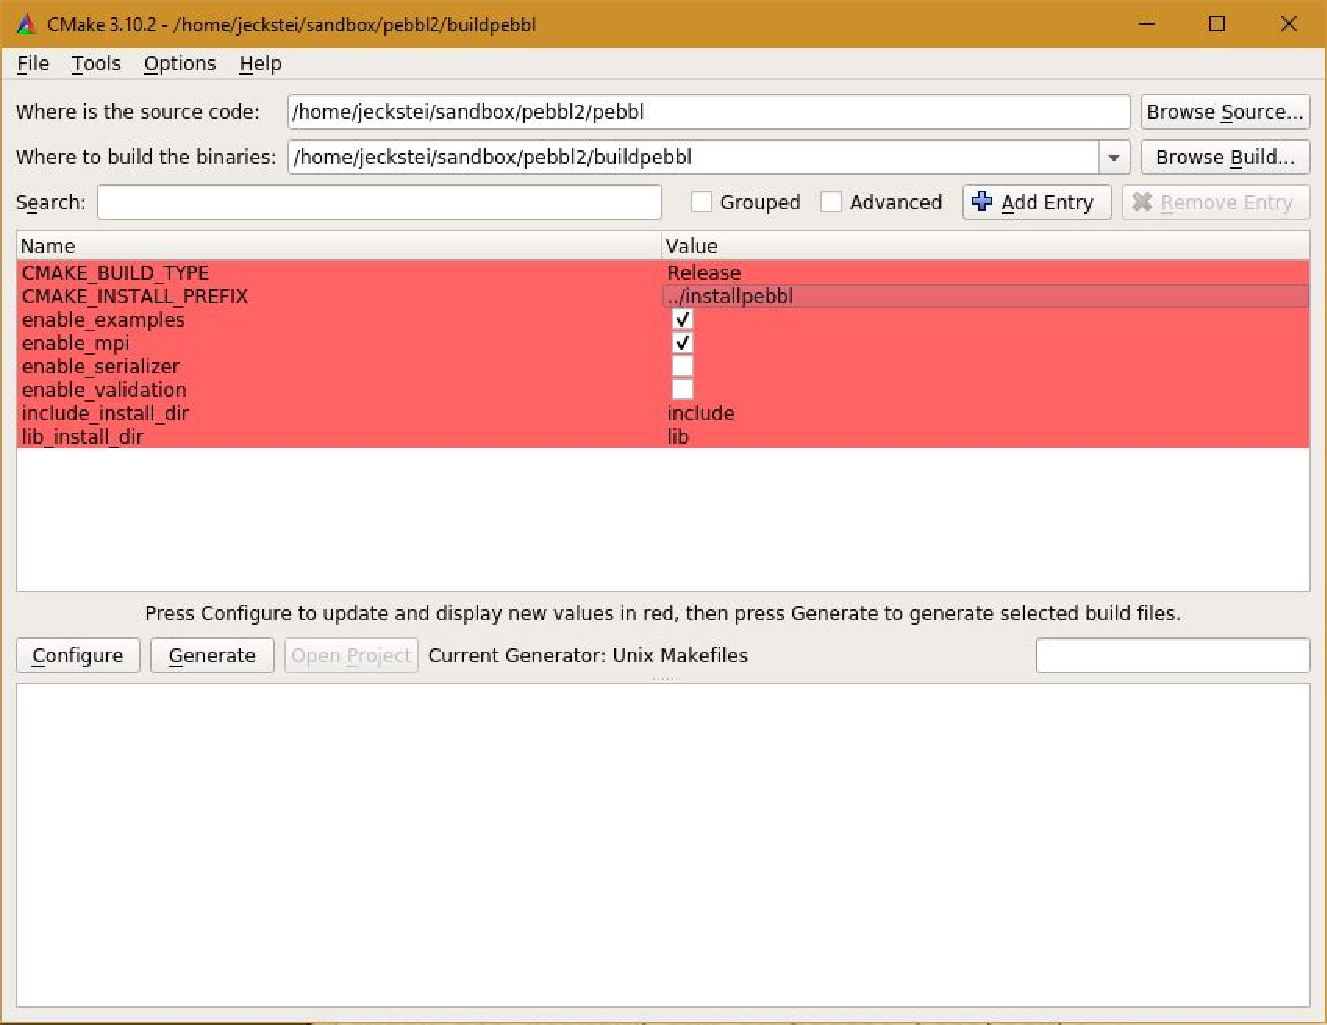
\includegraphics[height=0.45\textheight]{cmake3}
\vspace{-0.3in}
\end{center}{}
\caption{Appearance of \texttt{cmake-gui} after selecting (sample)
configuration options.
  \label{fig:cmake3}}
\end{figure}

Figure~\ref{fig:cmake3} shows the appearance of \texttt{cmake-gui} after
enabling MPI and selecting \texttt{installpebbl} (at the same level as
\texttt{pebbl} and \texttt{buildpebbl}) as the installation target directory.
Press the ``Configure'' button again, and the message pane at the bottom of
the \texttt{cmake-gui} window should the messages shown in
Figure~\ref{fig:cmake4}.  Press the ``Configure'' button once more, and you
should see the messages ``MPI Enabled'' and ``Configuring done'', as shown in
Figure~\ref{fig:cmake5}.  This status indicates that \texttt{cmake} is ready
to generate makefiles.  Press the ``Generate'', after which ``Generating
done'' should appear in the message pane.  At this point, PEBBL has been
configured; you may close the \texttt{cmake-gui} window.

\begin{figure}[tpb]
\begin{center}
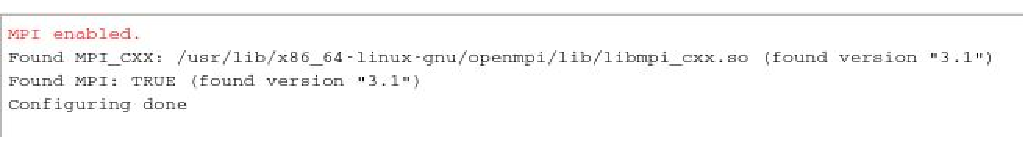
\includegraphics[width=0.8\textwidth]{cmake4}
\vspace{-0.3in}
\end{center}{}
\caption{Appearance of lower \texttt{cmake-gui} pane after second
configuration iteration.
  \label{fig:cmake4}}
\end{figure}

\begin{figure}[tpb]
\begin{center}
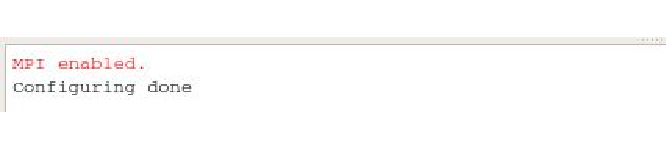
\includegraphics[width=0.5\textwidth]{cmake5}
\vspace{-0.3in}
\end{center}{}
\caption{Appearance of lower \texttt{cmake-gui} pane after third
configuration iteration (indicating that it is ready generate makefiles).
  \label{fig:cmake5}}
\end{figure}

\subsubsection{Configuring with \texttt{ccmake}}
The \texttt{cmake-gui} configuration process requires an X display.  If an X
display connection is not available or practical, PEBBL may instead by
configured using the \texttt{ccmake} terminal-interface tool or by issuing
\texttt{cmake} shell commands.  This section describes the \texttt{ccmake}
configuration procedure.

You initiate \texttt{ccmake} configuration much as with \texttt{cmake-gui}.

\textbf{FILL THIS IN}

\subsection{Compiling and installing}
Once the \texttt{cmake} configuration process is complete (using either
\texttt{cmake-gui} or \texttt{ccmake}), you compile PEBBL by simply issuing
the command \texttt{make} in the \texttt{buildpebbl} directory.  The resulting
output should have the following appearance:
{\footnotesize
\begin{verbatim}
Scanning dependencies of target pebbl
[  1%] Building CXX object src/pebbl/CMakeFiles/pebbl.dir/bb/branching.cpp.o
[  2%] Building CXX object src/pebbl/CMakeFiles/pebbl.dir/bb/loadObject.cpp.o
[  3%] Building CXX object src/pebbl/CMakeFiles/pebbl.dir/bb/pebblBase.cpp.o
[  4%] Building CXX object src/pebbl/CMakeFiles/pebbl.dir/bb/pebblParams.cpp.o
[  5%] Building CXX object src/pebbl/CMakeFiles/pebbl.dir/comm/MessageID.cpp.o
[  6%] Building CXX object src/pebbl/CMakeFiles/pebbl.dir/comm/coTree.cpp.o
\end{verbatim}
\vspace{-1.3ex}
$\qquad\vdots$
\begin{verbatim}
[ 95%] Building CXX object src/pebbl/example/CMakeFiles/commTest.dir/parKnapsack.cpp.o
[ 96%] Building CXX object src/pebbl/example/CMakeFiles/commTest.dir/serialKnapsack.cpp.o
[ 97%] Linking CXX executable commTest
[ 97%] Built target commTest
Scanning dependencies of target lipshitzian
[ 98%] Building CXX object src/pebbl/example/CMakeFiles/lipshitzian.dir/lipshitzian.cpp.o
[100%] Linking CXX executable lipshitzian
[100%] Built target lipshitzian
\end{verbatim}
}

You may accelerate the compilation process by using the \texttt{-j} option of
\texttt{make} to use multiple parallel threads.  For example, on a system with
8 processor cores, you could issue the command
\begin{codeblock}
make -j 8
\end{codeblock}
which would attempt to use 8 processes in parallel to speed up the compilation.

\textbf{Discuss make install and location of files}

\textbf{Test commands knapsack}

\textbf{How to set up makefiles for applications -- maybe defer until later?}
